\begin{figure}
    \caption{Evolución de la tarifa nominal del impuesto sobre la renta de personas jurídicas*}
    \label{fig:citrate}
    \centering
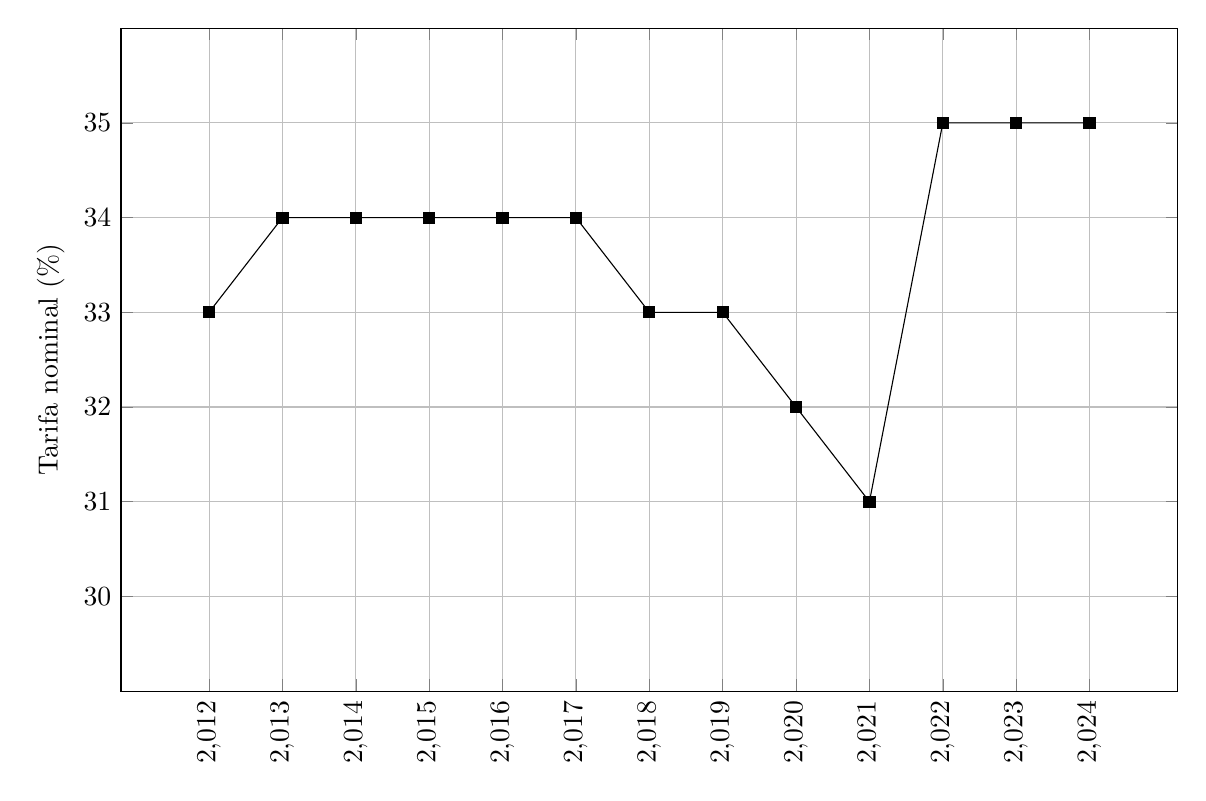
\begin{tikzpicture}
\begin{axis}[
    width=15cm,
    height=10cm,
%    xlabel={Año},
    ylabel={Tarifa nominal (\%)},
    grid=major,
    xtick=data,
    x tick label style={rotate=90, anchor=east},
    ymin=29,
    ymax=36,
    ytick={30,31,32,33,34,35},
    legend pos=south east
]

\addplot[mark=square*] coordinates {
%    (2011, 33)
    (2012, 33)
    (2013, 34)
    (2014, 34)
    (2015, 34)
    (2016, 34)
    (2017, 34)
    (2018, 33)
    (2019, 33)
    (2020, 32)
    (2021, 31)
    (2022, 35)
    (2023, 35)
    (2024, 35)
};

\end{axis}
\end{tikzpicture}
%\vspace{0.1cm}
%\par \footnotesize{*Incluye 9\% del CREE entre el 2013 y 2016}
\vspace{0.1cm}
\par \footnotesize{*Incluye 9\% del CREE entre 2013 y 2016}
\vspace{0.1cm}
\par \footnotesize{\textit{Fuente: Elaboración propia.}}
\end{figure}
